Pour l'existence d'une solution, nous allons devoir manipuler des \ncycles, définis ci-après, qui sont des objets plus souples que les polygones.


% ----------------------- %


\begin{defi}
    Pour $n \in \NN_{\geq3}$ uniquement, un \focus{\ncycle} désigne une liste ordonnée de $n$ points du plan, les répétitions étant possibles.
    Nous noterons $A_1 A_2 \cdots A_n$ un \ncycle,
    et appellerons
    \og \emph{sommets}\fg\ du \ncycle\ les points $A_i$ pour $i \in \ZintervalC{1}{n}$,
    où $A_1$ sera dit \focus{origine} du \ncycle.
\end{defi}


\begin{defi}
    Pour tout \ncycle\ $A_1 A_2 \cdots A_n$, on définit $\big( \primeit{A}_i \big)_{i \in \ZZ}$ comme étant $n$-périodique, et vérifiant $\primeit{A}_{i} = A_i$ sur $\ZintervalC{1}{n}$.%
    \footnote{
        Cette suite périodique va nous simplifier la vie dans l'écriture des énoncés et des preuves.
    }
\end{defi}


\begin{defi}
    Les \focus{côtés} d'un \ncycle\ $\setproba{L} = A_1 A_2 \cdots A_n$ sont les segments
    $[\primeit{A}_i \primeit{A}_{i+1}]$ pour $i \in \ZintervalC{1}{n}$,
    et
    la \focus{longueur} de $\setproba{L}$ est définie par $\cyclelen{\setproba{L}} = \dsum_{i=1}^{n} \primeit{A}_i \primeit{A}_{i+1}$.
\end{defi}


\begin{defi}
    Un \ncycle\ est \focus{dégénéré} s'il a, au moins, trois sommets consécutifs alignés,
    et il est dit \focus{totalement dégénéré} si tous ses sommets sont alignés.
\end{defi}


% ----------------------- %


\begin{defi}
    Un \focus{\ngone} indique un \ncycle\ non dégénéré n'admettant aucun couple de côtés non contigus et sécants,
    et
    un \focus{\ngone\ croisé} désigne un \ncycle\ non dégénéré qui n'est pas un \ngone.%
    \footnote{
        Bien retenir que, par définition, un \ngone\ n'est jamais croisé.
    }
    La longueur d'un \ngone, croisé ou non, est aussi appelée \focus{périmètre}.
\end{defi}


\begin{remark}
    Voici des exemples pour clarifier le vocabulaire.
    %
    \begin{center}
        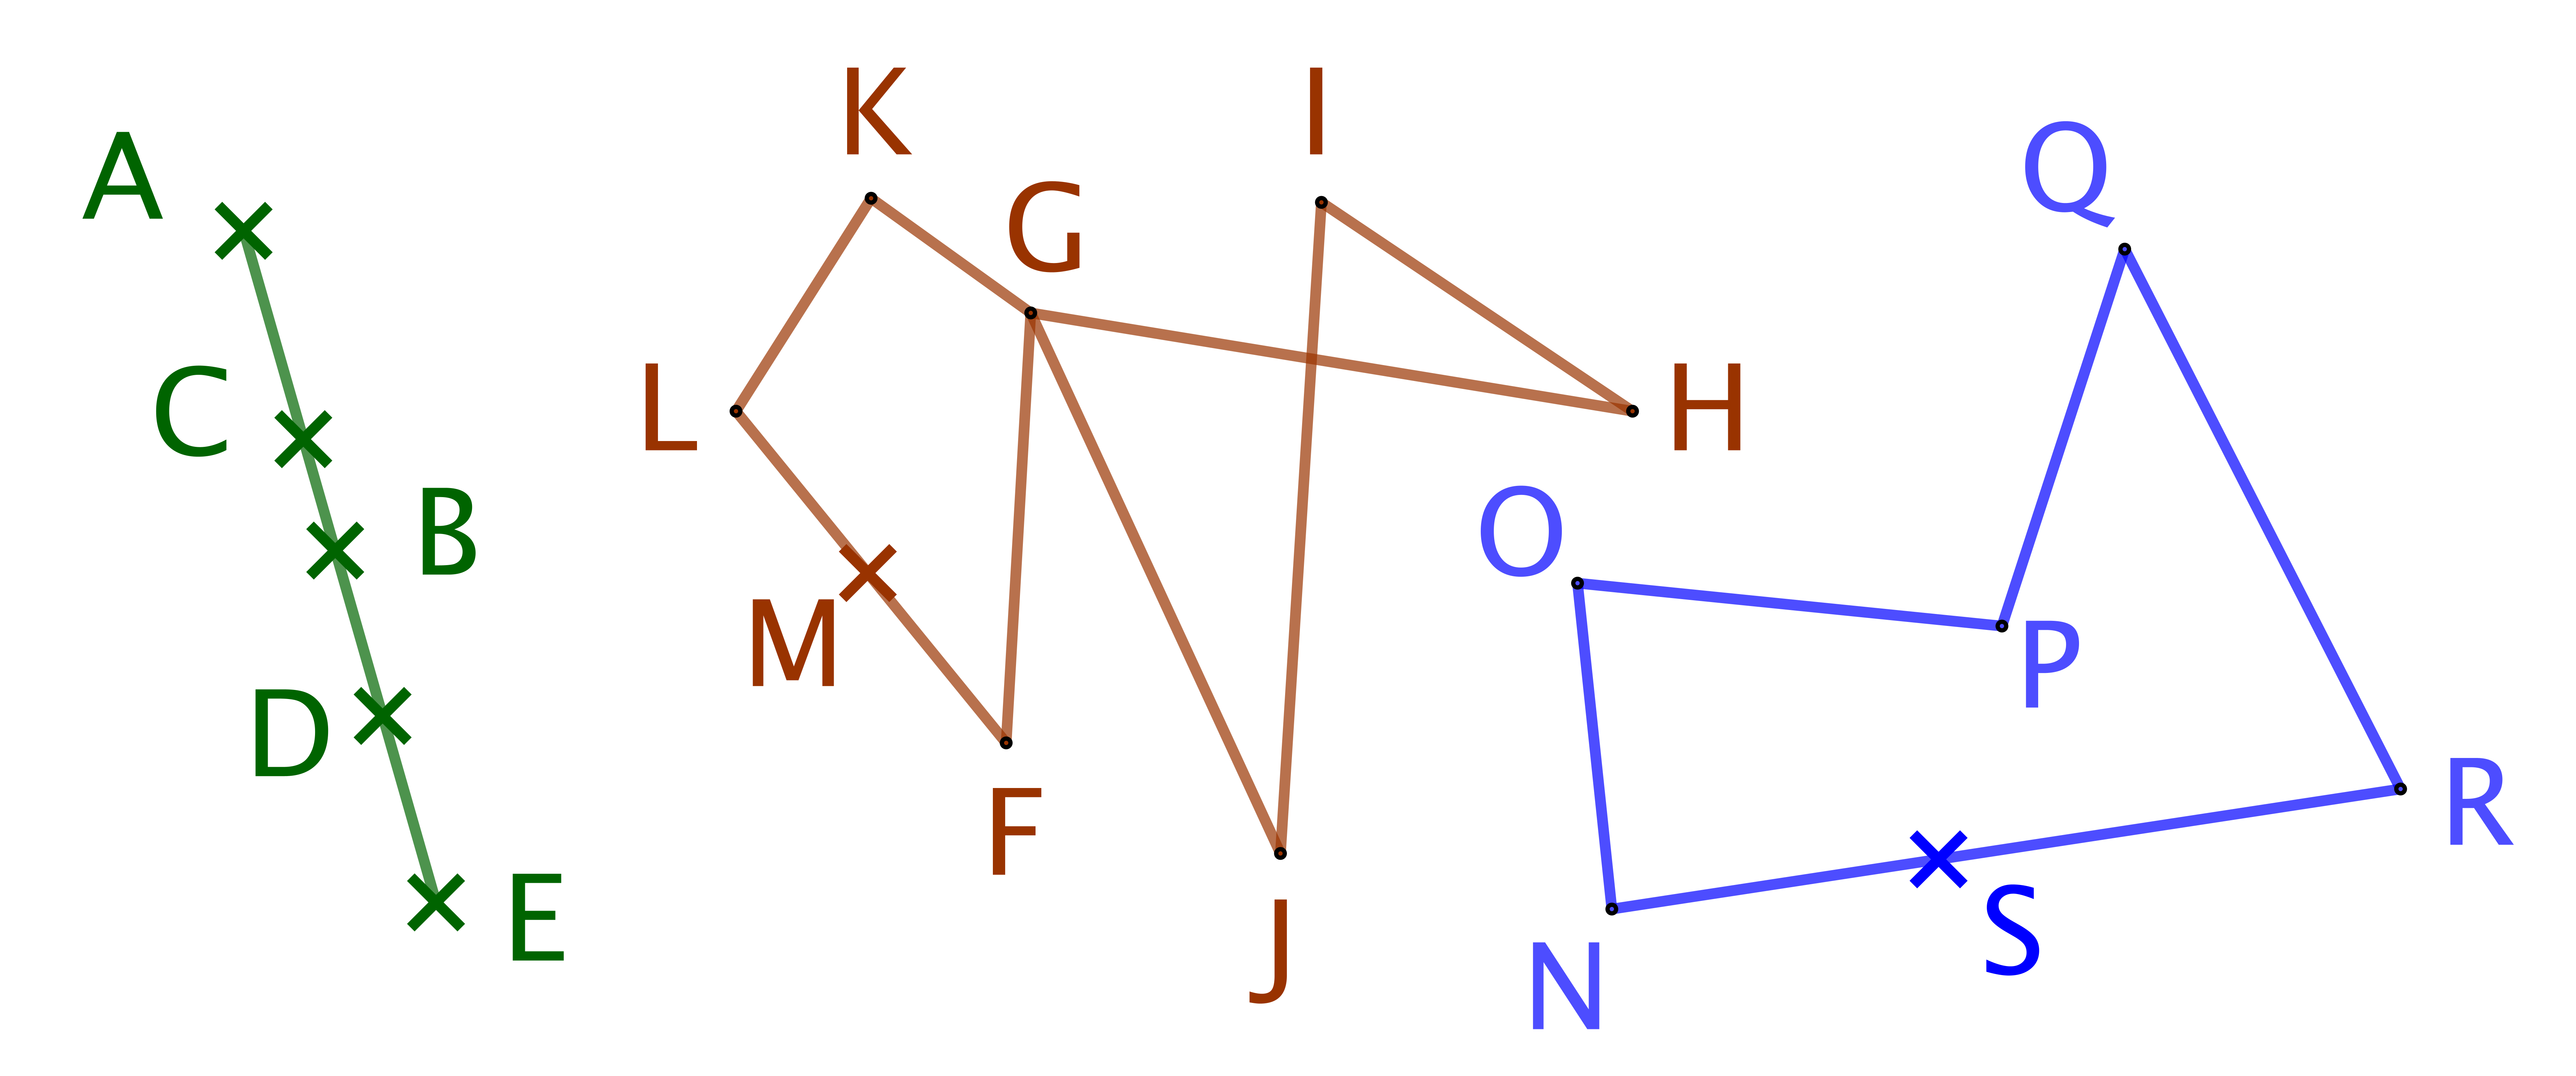
\includegraphics[scale=.3]{some-ncycles-ngones.png}
    \end{center}

    $ABCDE$ est un \xcycle{5} totalement dégénéré,
    $FGHIJGKLM$ un \xcycle{9} dégénéré sans être un \xgone{9},
    $NOPQRS$ un \xcycle{6} dégénéré sans être un \xgone{6},
    $FGHIJGKL$ un \xgone{8} croisé,
    et enfin
    $NOPQR$ un \xgone{5}.
\end{remark}


% ----------------------- %


\begin{defi}
    Un \ngone, croisé ou non, est dit \focus{équilatéral} si tous ses côtés sont égaux.
\end{defi}


\begin{defi}
    Un \ngone, croisé ou non, est dit \focus{équiangle} si tous ses angles au sommet sont de même mesure.
\end{defi}


\begin{defi}
    Un \ngone, croisé ou non, est dit \focus{régulier} s'il est équiangle et équilatéral.
\end{defi}


\begin{remark}
    Un losange non carré est un \nequi\ non régulier, et un rectangle non carré est un \niso\ non régulier.
\end{remark}


\begin{remark}
    Il existe des \nregs\ et croisés.

    \vspace{-1.5em}

    \begin{multicols}{2}
        \small\itshape\centering

        \null\vfill

        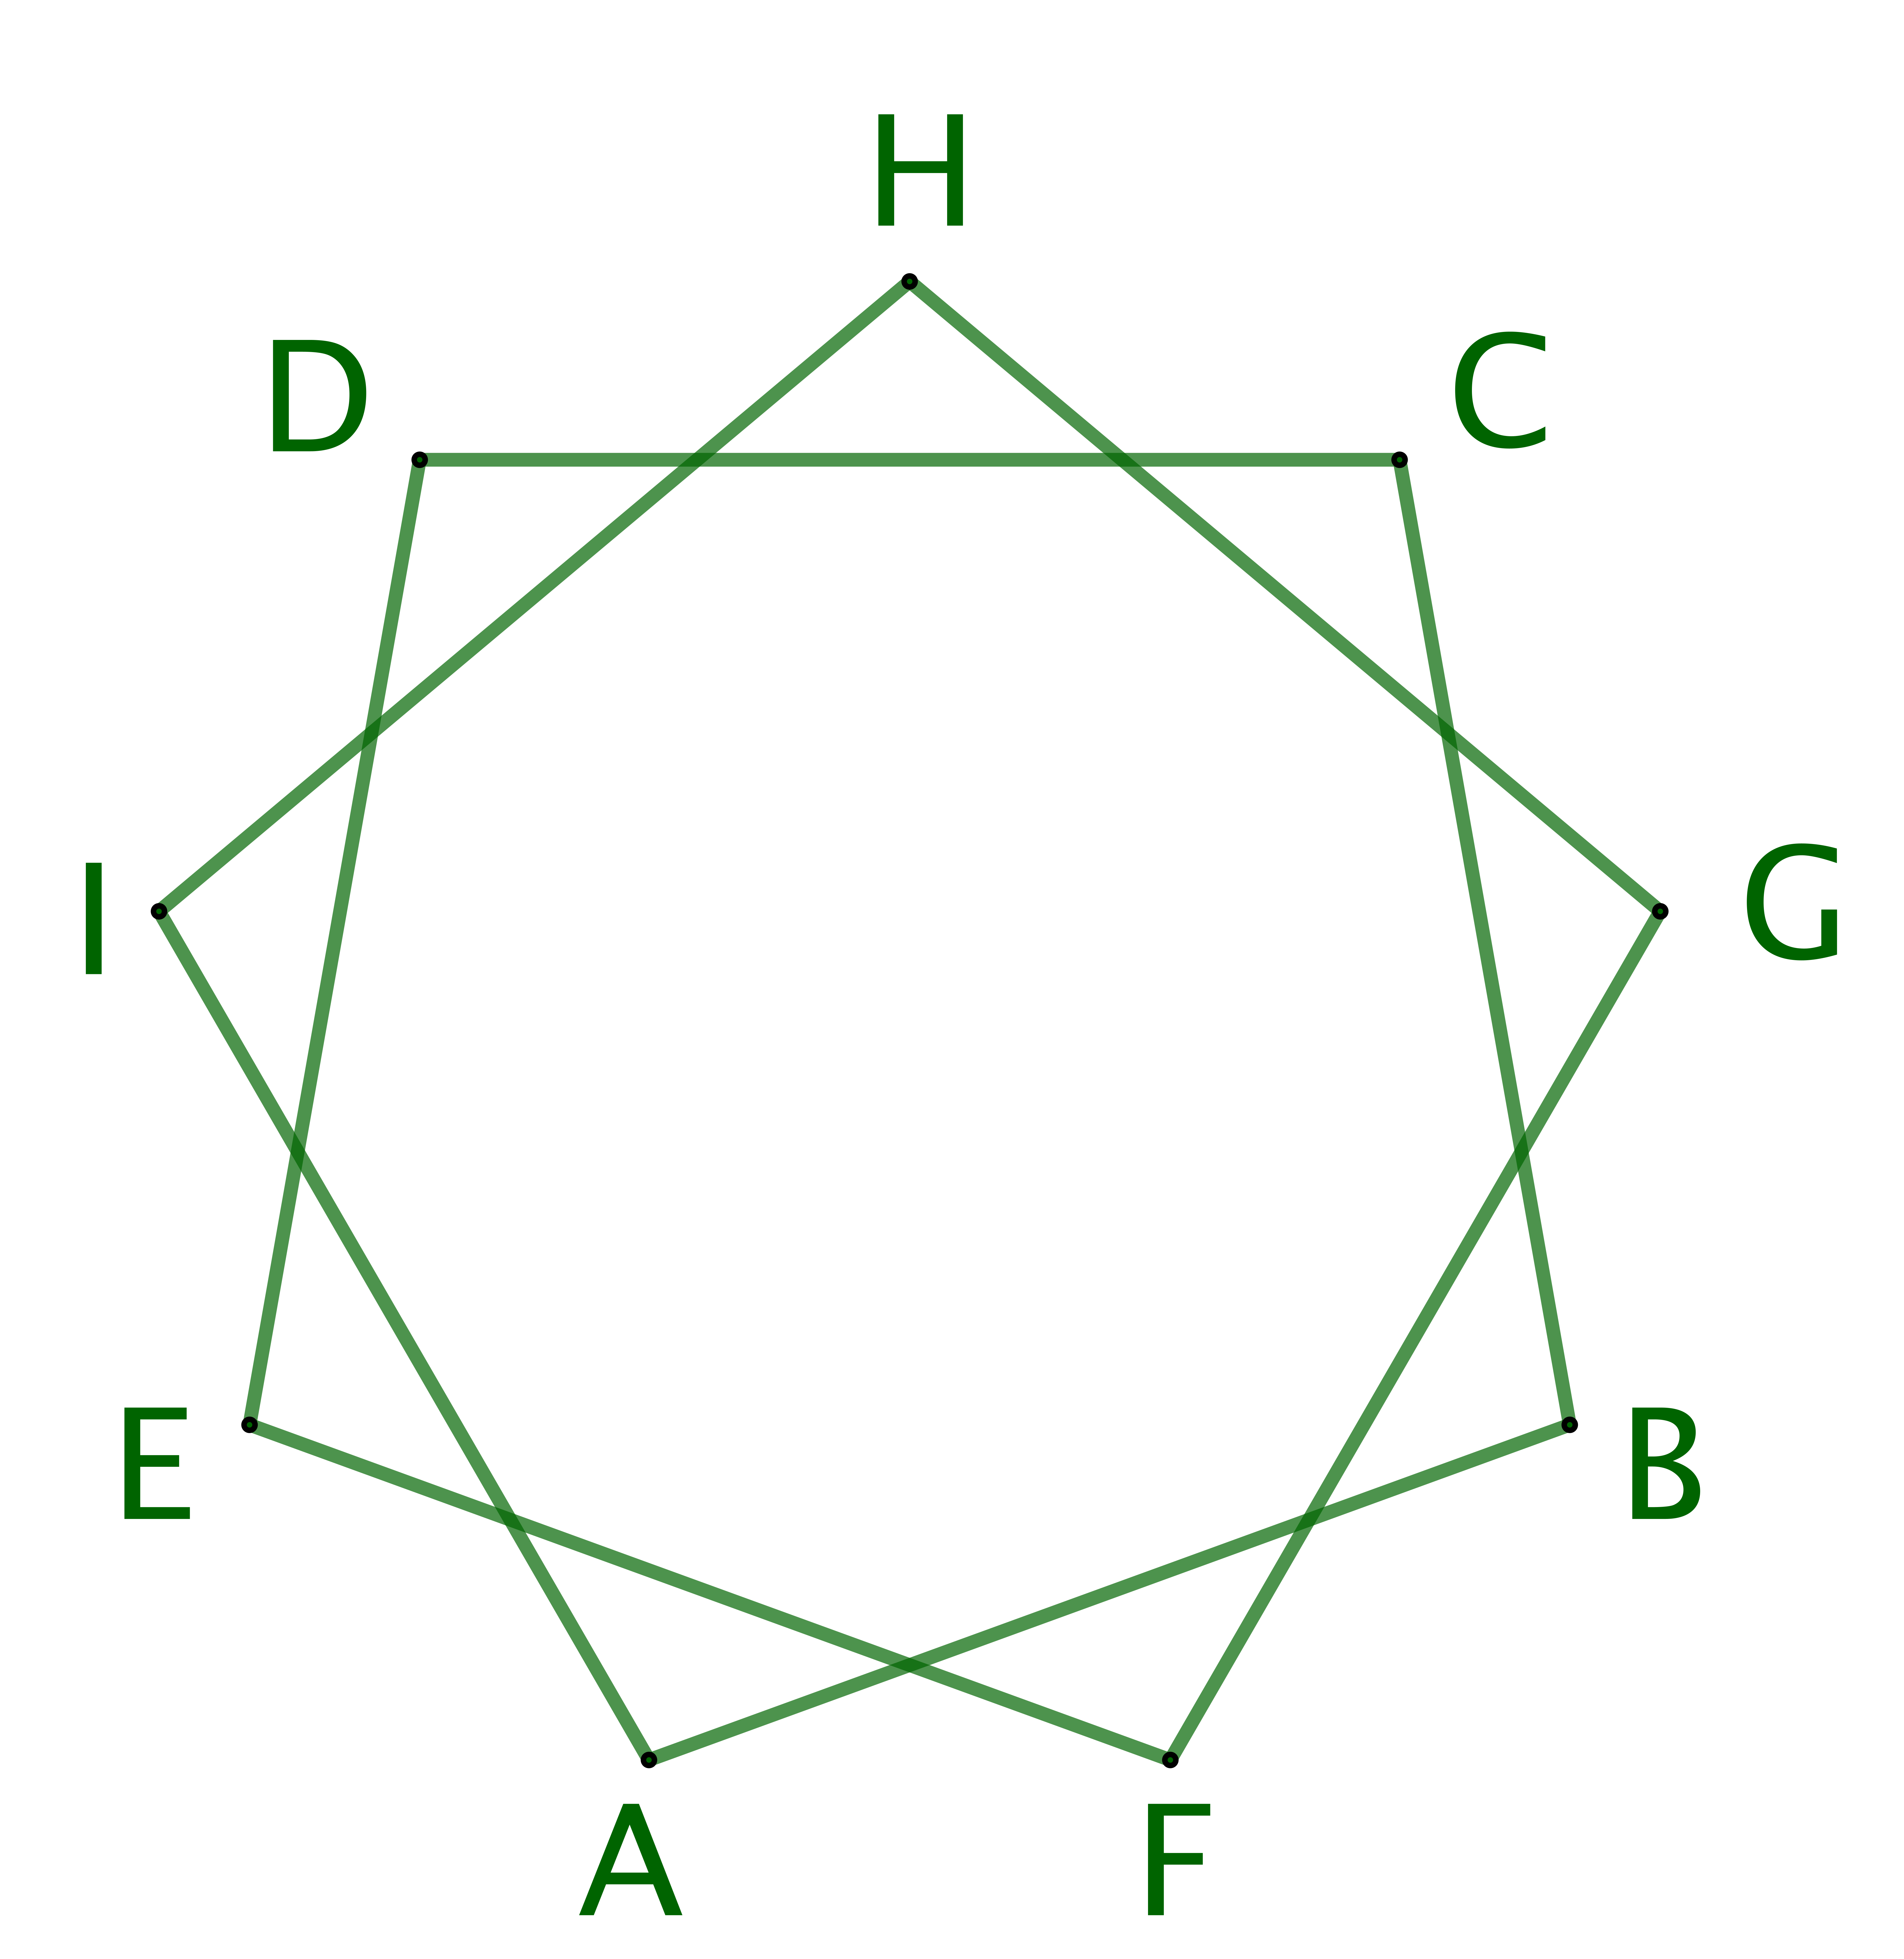
\includegraphics[scale=.175]{9-iso-non-conv.png}

        \smallskip
        Un ennéagone régulier croisé dit étoilé.%
        \footnote{
            La construction se fait via $AFBGCHDIE$ qui est un \xreg{9} en reliant un sommet sur deux. Elle se généralise à tout \nreg\ pour $n$ impair.
        }

%        \vfill\null

        \columnbreak

        \null\vfill

        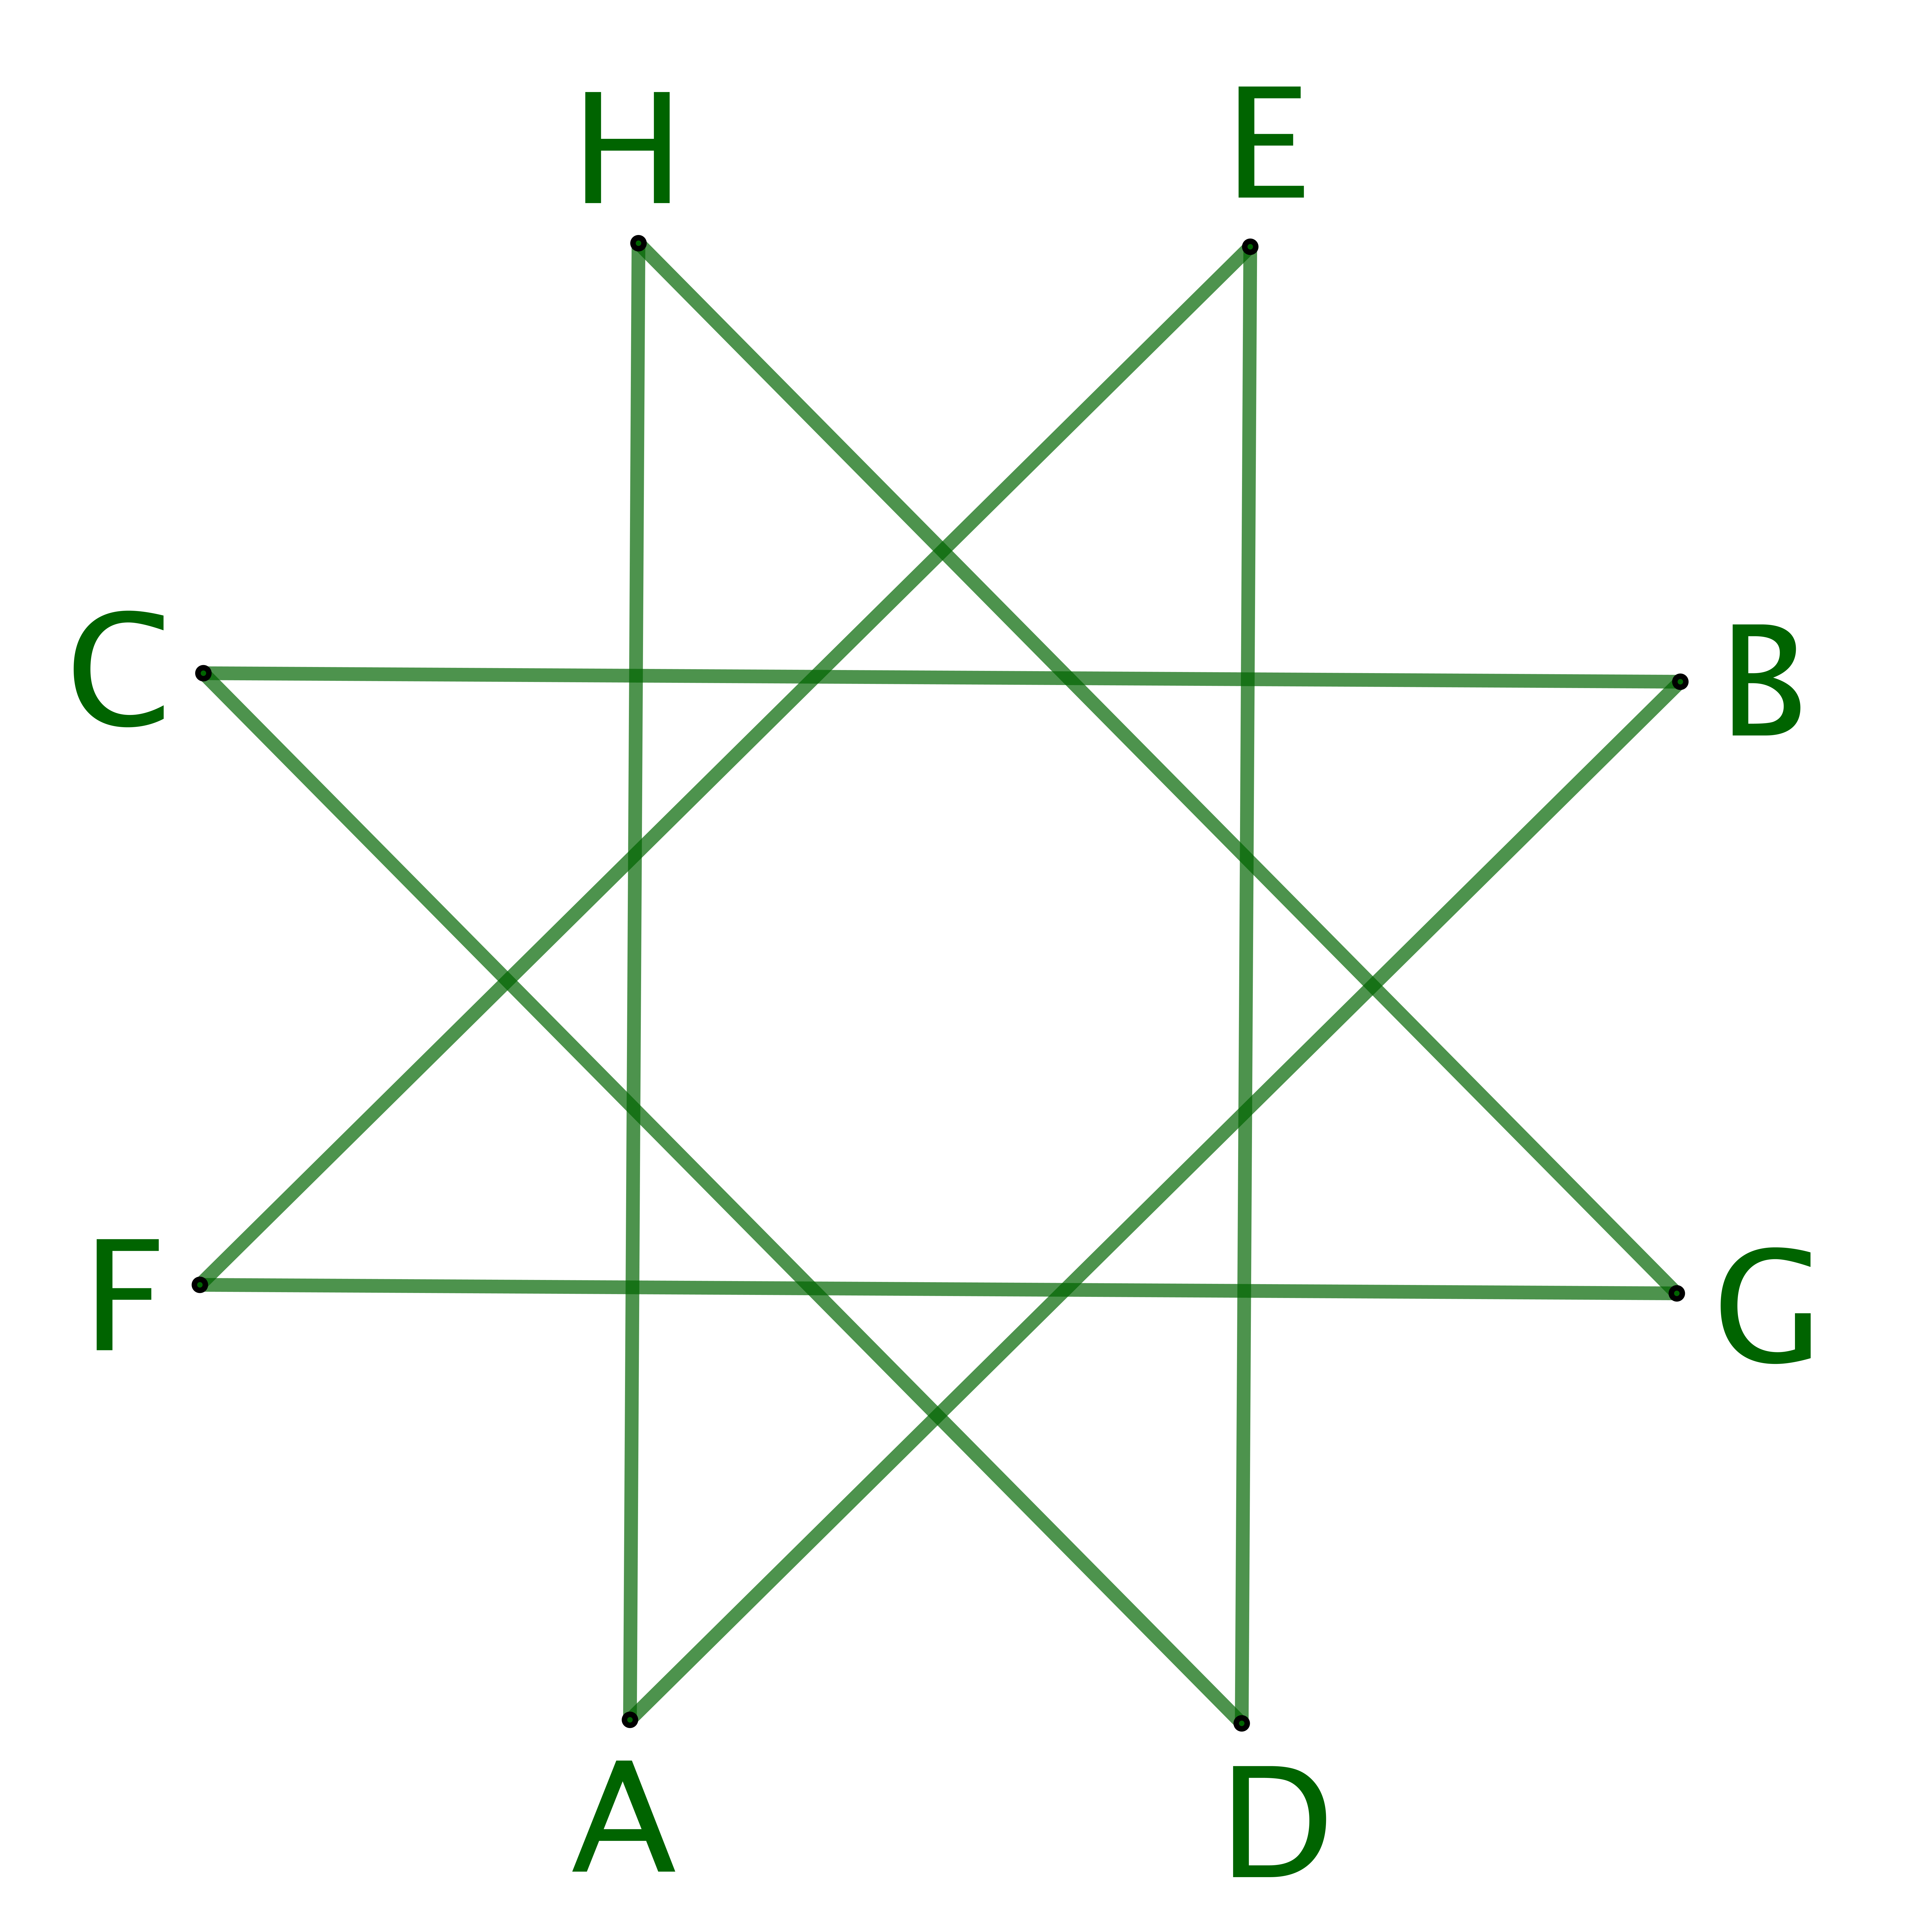
\includegraphics[scale=.175]{8-iso-non-conv.png}

        \smallskip
        Un octogone régulier croisé dit étoilé.%
        \footnote{
            La construction se fait via le \xreg{8} intérieur en prolongeant les côtes. Elle se généralise à tout \nreg\ pour $n$ pair.
        }

%        \vfill\null
    \end{multicols}
\end{remark}
